\documentclass{standalone}
\usepackage{tikz}
\usepackage{xcolor}
\usetikzlibrary{circuits.ee.IEC, positioning, shadows.blur, shapes, decorations.pathmorphing, backgrounds}

% Definindo as cores neon
\definecolor{neoncyan}{RGB}{0, 255, 255}
\definecolor{neonorange}{RGB}{255, 90, 0}
\definecolor{darkblue}{RGB}{10, 15, 30}

% Define the Sun as a TikZ style
\tikzset{
    % This code defines a reusable TikZ style called "sun" that creates a stylized sun graphic,
    % hat can be applied to TikZ nodes or paths.
    sun/.style={
        postaction={
             % O decorate ativa o mecanismo de decoração do TikZ, indicando que o caminho (path) ou 
             % elemento será modificado por algum tipo de decoração. Ele transforma o caminho original 
             % ao qual é aplicado, permitindo que o decorador especificado (neste caso, markings) 
             % seja aplicado ao caminho. Também servindo como como uma ponte entre o elemento TikZ e 
             % a decoração específica definida no parâmetro decoration={...}.
             % decorate trabalha em conjunto com a decoração markings para permitir a colocação de um 
             % elemento gráfico complexo (o sol) em um ponto específico do caminho. Sem o decorate, 
             % as instruções de decoração seriam ignoradas e o sol não seria desenhado quando você 
             % aplicasse o estilo a um nó. Em resumo, é "interruptor" que ativa o sistema de decoração 
             % do TikZ, permitindo que elementos gráficos complexos (como seu sol) sejam adicionados a 
             % caminhos ou nós em posições específicas.
            decorate,
            decoration={
                markings,
                % This instruction, which places the sun graphic at the beginning (position 0) of 
                % whatever path it's applied to.
                mark=at position 0 with {
                    \fill[darkblue] (0,0) circle (1.); % clean backdrop
                    % Draw the rays: First, the code draws 16 rays emanating from the origin (0,0) 
                    % using a \foreach loop. Each ray is drawn with the neon orange color and 
                    % has a width of 1.5pt. The rays are evenly spaced in a 360° circle 
                    % (each at 22.5° intervals) and extend 1.5 units from the center.
                    \foreach \i in {0,...,15} {
                        \draw[neonorange, line width=1.5pt] (0,0) -- ++(\i*22.5:0.9);
                    }
                    % Draw the kernel: Second, the "kernel" of the sun is drawn as two concentric circles. 
                    % Both circles are outlined in neon orange with a line width of 1.5pt and filled with dark blue. 
                    % The outer circle has a radius of 1 unit, while the inner circle has a radius of 0.8 units, 
                    % creating a ring-like appearance.
                    \draw[neonorange, line width=1.5pt, fill=darkblue] (0,0) circle (.6);
                    \draw[neonorange, line width=1.5pt, fill=darkblue] (0,0) circle (.4);
                }
            }
        }
    }
}

%% Eye style definition
\tikzset{
    eye/.style={
        postaction={
            decorate,
            decoration={
                markings,
                mark=at position 0 with {
                    \fill[darkblue] (0,0) ellipse (2cm and 1.5cm); % clean backdrop
                    \draw[neonorange, line width=1.5pt] (0,0) circle (0.5); % Iris
                    \draw[neonorange, line width=1.5pt] (-1.9,0.1) -- (-1.5,0.1) .. controls (-0.5,1) and (0.5,1) .. (1.5,0.1) -- (1.9,0.1); % Upper eye contour
                    \draw[neonorange, line width=1.5pt] (1.9,-0.1) -- (1.5,-0.1) .. controls (0.5,-1) and (-0.5,-1) .. (-1.5,-0.1) -- (-1.9,-0.1); % Lower eye contour
                    \draw[neonorange, line width=1.5pt] (0,-0.85) -- (0,-1.4); % Risk down
                    \draw[neonorange, line width=1.5pt] (0.9,0.8) arc (20:160:1cm and 0.4cm); % Arc above the circle
                }
            }
        }
    }
}

% Box for keyboard shortcuts
\tikzset{
    box/.style 2 args={
        minimum width=#2,
        % Passing the width as the second parameter
        minimum height=4.cm,
        align=center,
        % The append after command is a powerful TikZ option that executes additional commands after a node is created. It's being used here to augment the node with a custom style shape.
        append after command={
            % creates a block where raw PGF commands (TikZ's underlying engine) can be used. 
            \pgfextra{
                % The code first retrieves the node's dimensions using \pgfkeysgetvalue, storing the width and height in \boxwidth and \boxheight respectively.
                \pgfkeysgetvalue{/pgf/minimum width}{\boxwidth}
                \pgfkeysgetvalue{/pgf/minimum height}{\boxheight}
                % Define the shift to outset the box's content, creating a 'hexagon'-like appearance in the corners.
                \def\shift{0.6cm}
                % External contour of the box with neon effect
                \draw[#1, line width=2pt, fill=darkblue]
                    (\tikzlastnode.south west) --
                    ([xshift=-\shift, yshift=\shift]\tikzlastnode.south west) -- 
                    ([xshift=-\shift, yshift=-\shift]\tikzlastnode.north west) -- 
                    (\tikzlastnode.north west)--
                    (\tikzlastnode.north east) -- 
                    ([xshift=\shift, yshift=-\shift]\tikzlastnode.north east) -- 
                    ([xshift=\shift, yshift=\shift]\tikzlastnode.south east) --
                    (\tikzlastnode.south east) -- cycle;
                % Internal contour of the box with neon effect
                \draw[#1, line width=1.5pt]
                    ([yshift=0.3*\shift]\tikzlastnode.south west) --
                    ([xshift=-0.7*\shift, yshift=\shift]\tikzlastnode.south west) -- 
                    ([xshift=-0.7*\shift, yshift=-\shift]\tikzlastnode.north west) -- 
                    ([yshift=-0.3*\shift]\tikzlastnode.north west)--
                    ([yshift=-0.3*\shift]\tikzlastnode.north east) -- 
                    ([xshift=0.7*\shift, yshift=-\shift]\tikzlastnode.north east) -- 
                    ([xshift=0.7*\shift, yshift=\shift]\tikzlastnode.south east) --
                    ([yshift=0.3*\shift]\tikzlastnode.south east) -- cycle;
            }
        }
    }
}

% Define a reusable keyboard shortcut key style
\tikzset{
    key/.style 2 args={
        draw=#1,
        rounded corners,
        line width=1.5pt,
        minimum width=#2,
        minimum height=1.5cm,
        align=center,
        text=white,
        font=\sffamily\bfseries\Large,
        fill=darkblue
    }
}

% Define a shortcut box command
\newcommand{\shortcutbox}[5]{
    % #1: position (x,y)
    % #2: border color
    % #3: action text
    % #4: shortcut key
    % #5: minimum width bigger box
    \node[box={#2}{#5}] at (#1) {};
    \node[text=#2!50, font=\sffamily\bfseries\Large, align=center] at ([yshift=1.cm]#1) {#3};
    \node[key={#2}{0.8*#5}] at ([yshift=-0.8cm]#1) {#4};
}


\begin{document}
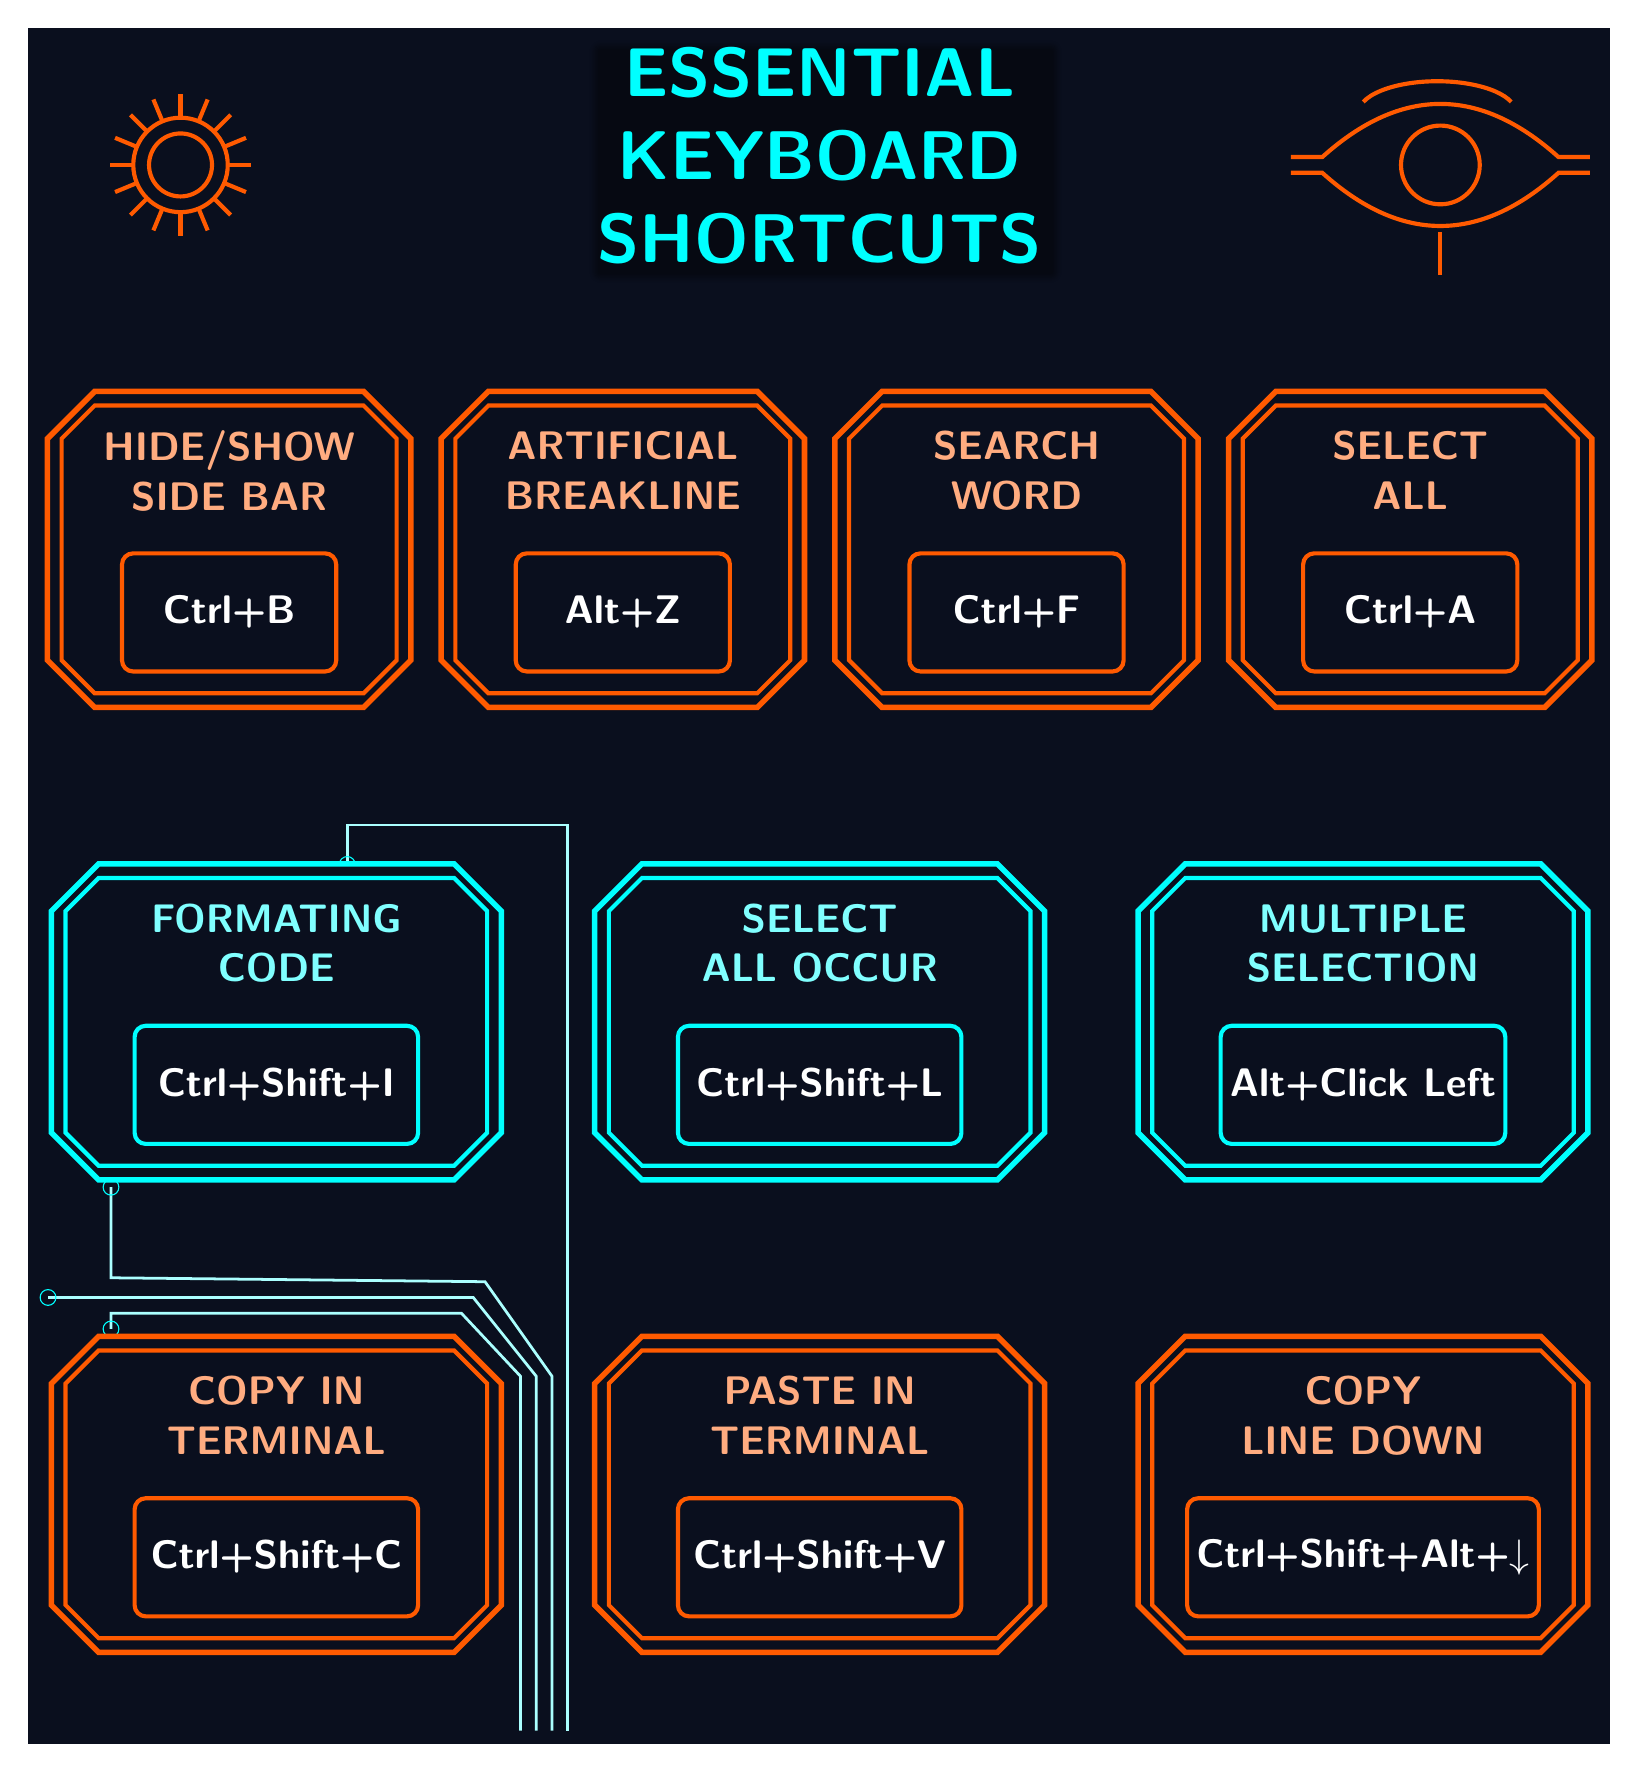
\begin{tikzpicture}[
		% Defines a style for the background rectangle of a TikZ element in LaTeX.
		% background rectangle refers to the rectangle that serves as the background 
		% for certain TikZ elements (often used with show background rectangle option).
		% The /.style={...} is how TikZ defines styles - it's creating or modifying a property.
		background rectangle/.style={fill=darkblue},
		% The option show background rectangle is a TikZ directive that enables display of a 
		% background rectangle for your diagram.
		% When included in a TikZ picture's options list, this command instructs TikZ to draw a rectangle that encompasses all the content of the picture. It functions as a container or 
		% backdrop for your entire diagram. 
		show background rectangle
	]
	% Desenho dofundo com circuitos
    % Circuit with neon effect - vertical line left
    \draw[neoncyan!33, line width=1pt] (6.2,0) -- (6.2,4.5) -- (5.45,5.3) -- (5.45,5.3) -- (1,5.3) -- (1,5.3) -- (1,5.1); 
    \draw[neoncyan]  (1,5.1) circle (0.1); % Circle
    \draw[neoncyan!33, line width=1pt] (6.4,0) -- (6.4,4.5) -- (5.6,5.5) -- (5.45,5.5) -- (1,5.5) -- (0.2,5.5); 
    \draw[neoncyan]  (0.2,5.5) circle (0.1); % Circle
    \draw[neoncyan!33, line width=1pt] (6.6,0) -- (6.6,4.5) -- (5.75,5.7) -- (5.75,5.7) -- (1,5.75) -- (1,6.9); 
    \draw[neoncyan]  (1,6.9) circle (0.1); % Circle
    \draw[neoncyan!33, line width=1pt] (6.8,0) -- (6.8,11.5) -- (4,11.5) -- (4,11.); 
    \draw[neoncyan]  (4,11) circle (0.1); % Circle

	% Elementos simbólicos (olho, sol, etc)
	%% Draw the sun at position (2,18)
	\path (2,20) node[sun] {};
	%% Draw the eye at position (18,18)
	\path (18,20) node[eye] {};

	% Título em neon
	\node[align=center, font=\sffamily\bfseries\Huge, text=neoncyan, blur shadow={shadow blur steps=5,shadow blur extra rounding=2pt}]
	at (10,20) {ESSENTIAL\\KEYBOARD\\SHORTCUTS};

    % First row using relative positioning
	% (x,y)(color)(text)(shortcut)
    % Define anchor position for first row
    \coordinate (firstbox) at (2.5,15);
    \def\hstep{5.cm} % Horizontal spacing between boxes
    \def\boxwidth{3.4cm} % Common width for all boxes

    \shortcutbox{firstbox}{neonorange}{HIDE/SHOW\\SIDE BAR}{Ctrl+B}{\boxwidth}
    \shortcutbox{$(firstbox)+(1*\hstep,0)$}{neonorange}{ARTIFICIAL\\BREAKLINE}{Alt+Z}{\boxwidth}
    \shortcutbox{$(firstbox)+(2*\hstep,0)$}{neonorange}{SEARCH\\WORD}{Ctrl+F}{\boxwidth}
    \shortcutbox{$(firstbox)+(3*\hstep,0)$}{neonorange}{SELECT\\ALL}{Ctrl+A}{\boxwidth}

    % Second row using relative positioning
    \coordinate (secondbox) at (3.1,9);
    \def\hstep{6.9cm} % Horizontal spacing between boxes
    \def\boxwidth{4.5cm}

	\shortcutbox{secondbox}{neoncyan}{FORMATING\\CODE}{Ctrl+Shift+I}{\boxwidth}
	\shortcutbox{$(secondbox) + (1*\hstep,0)$}{neoncyan}{SELECT\\ALL OCCUR}{Ctrl+Shift+L}{\boxwidth}
	\shortcutbox{$(secondbox) + (2*\hstep,0)$}{neoncyan}{MULTIPLE\\SELECTION}{Alt+Click Left}{\boxwidth}

    % Third row using relative positioning
    \coordinate (thirdbox) at (3.1,3);
	\shortcutbox{thirdbox}{neonorange}{COPY IN\\TERMINAL}{Ctrl+Shift+C}{\boxwidth}
	\shortcutbox{$(thirdbox) + (1*\hstep,0)$}{neonorange}{PASTE IN\\TERMINAL}{Ctrl+Shift+V}{\boxwidth}
	\shortcutbox{$(thirdbox) + (2*\hstep,0)$}{neonorange}{COPY\\LINE DOWN}{Ctrl+Shift+Alt+$\downarrow$}{\boxwidth}
	% Adicionar mais símbolos e linhas de circuitos
	% ...

\end{tikzpicture}
\end{document}